\documentclass[12pt]{article}

%% page layout
\textheight 9in 
\textwidth 6.5in
\topmargin -0.5in
\oddsidemargin 0in
\evensidemargin 0in
%\hoffset=-0.5in
\voffset=-0.25in

%% packages
\usepackage{scrtime} % for \thistime (this package MUST be listed first!)
\usepackage{amsmath} % essential for cases environment
\usepackage{amsthm} % for theorems and proofs
\usepackage{amsfonts} % mathbb
\usepackage{graphics,graphicx}
\usepackage{multirow} % fancy tables
\usepackage{wasysym} % circle symbols (including half-filled circles)
\usepackage{enumerate} % fancier enumeration (e.g., a,b,c, ...)
%\usepackage{xcolor}
\usepackage{color}
\newcommand{\de}[1]{{\color{red}{\bfseries DE:} #1}}

%% for solutions to multiple choice questions:
\newcommand{\correct}{{\color{blue}\fbox{\color{red}\checkmark} }}

%% macros
\newcommand{\reals}{\mathbb{R}}
\newcommand{\term}[1]{{\bfseries\slshape #1}}
\newcommand{\Ker}{{\text{Ker}\,}}
\newcommand{\Range}{{\text{Range}\,}}
\newcommand{\diag}{{\text{diag}}}
\newcommand{\alg}{{\text{alg}}}
\newcommand{\geom}{{\text{geom}}}
\newcommand{\norm}[1]{\left\|#1\right\|}
\newcommand{\abs}[1]{\left|#1\right|}
\newcommand{\R}{{\cal R}}
\newcommand{\G}{{\cal G}}
\newcommand{\eps}{\varepsilon}
\newcommand{\B}{\cal B}
\newcommand{\Tinf}{T_\textrm{inf}}
\newcommand{\Shat}{{\hat{S}}}
\newcommand{\Ihat}{{\hat{I}}}
\newcommand{\ie}{\emph{i.e., }}
\newcommand{\eg}{\emph{e.g., }}
\newcommand{\Rlogo}{\protect
\includegraphics[height=2ex,keepaspectratio]{images/Rlogo.pdf}\xspace}
\newcommand{\XPPAUT}{\texttt{XPPAUT}\xspace}
\newcommand{\etal}{\textit{et al}.\xspace}
\newcommand\emphblue[1]{\emph{\color{blue}#1}}

%%%%%%%%%%%%%%%%%%%%%%%%%%%%
%% from feverpreamble.tex %%
%%%%%%%%%%%%%%%%%%%%%%%%%%%%

\usepackage{amssymb,latexsym,amsmath,setspace}
%%\usepackage[colorlinks,linkcolor=blue]{hyperref}
\usepackage[colorlinks=true,allcolors=blue]{hyperref}
%%\usepackage[colorlinks]{hyperref}
\usepackage{xspace}
\usepackage{graphics,graphicx}
\usepackage{subfigure}
\usepackage{lineno}
\usepackage{fancyhdr}
\usepackage[english]{babel}  %% for texi2dvi ~ bug
\usepackage[normalem]{ulem}
\usepackage{tikz} % http://www.texample.net/tikz/examples/tikzdevice-demo/
  % N.B. version 0.6.3 of tikzDevice from Rforge is required!!
%% improve figure caption typsetting:  (see ~/tex/caption.pdf for manual)
\usepackage[footnotesize,bf]{caption}
\usepackage{placeins} % \FloatBarrier

% citation macros
\newcommand{\citen}[1]{\cite{#1}}

% comment macros
\usepackage{color}
\newcommand{\comment}[3]{\textcolor{#1}{\textbf{[#2: }\textit{#3}\textbf{]}}}
\newcommand{\david}[1]{\comment{blue}{DE}{#1}}
\newcommand{\paul}[1]{\comment{cyan}{PA}{#1}}
\newcommand{\ben}[1]{\comment{magenta}{BB}{#1}}
\newcommand{\needref}{{\textcolor{red}{[NEED REF]}}}
\newcommand{\TBD}{{\textcolor{red}{{\bf TBD}}}}
% remove comments
%\renewcommand{\comment}[3]{\relax}
% remove section headings
%\def\subsubsection*#1{\relax\nobreak}

% other macros
\newcommand{\avg}[1]{{\left\langle#1\right\rangle}}
\newcommand{\var}[1]{\textrm{var}\left(#1\right)}
\newcommand{\sem}[1]{\textrm{sem}\left(#1\right)}
\newcommand{\natinf}{{\mathcal I}}
\newcommand{\find}{f_{\textrm{i}}}
\newcommand{\fpop}{f_{\textrm{p}}}
\newcommand{\logit}{\textrm{logit}}
\newcommand{\sign}{\textrm{sign}}
\newcommand{\logistic}{\textrm{logistic}}
\def\AJE{{\it American Journal of Epidemiology\/}}
\newcommand{\code}[1]{{\tt #1}}
\newcommand{\magcode}[1]{{\tt\color{magenta}#1}}
\newcommand{\redcode}[1]{{\tt\color{red}#1}}
\newcommand{\blackcode}[1]{{\tt\color{black}#1}}

%%%%%%%%%%%%%%%%%%%
%% JOURNAL NAMES %%
%%%%%%%%%%%%%%%%%%%
\def\PNAS{PNAS}
\def\JAMA{JAMA}
\def\BMB{{\it Bulletin of Mathematical Biology\/}}

% references
\newcommand{\eref}[1]{Equation~\eqref{E:#1}}
\newcommand{\fref}[1]{Figure~\ref{F:#1}}
\newcommand{\tref}[1]{Table~\ref{T:#1}}
\newcommand{\sref}[1]{\S\ref{S:#1}}
% other macros
\newcommand{{\Reff}}{{\mathcal{R}}_{\rm eff}}
\newcommand{{\Sinit}}{S_{\rm init}}
\newcommand{\supp}{Supplementary Information}
\newcommand{\StoppedHere}{\bigskip\bigskip{\textcolor{red}{\hrule\centerline{\bfseries STOPPED HERE}\hrule}}\bigskip\bigskip}
\newcommand{\colvec}[2]{\begin{pmatrix}#1\\#2\end{pmatrix}}
\newcommand{\diagmat}[3]{\begin{pmatrix}#1&0&0\\0&#2&0\\0&0&#3\end{pmatrix}}

\newcommand{\solution}[1]{{\hfill\break\vspace{-0.5\baselineskip}\break\color{blue}\emph{Solution: }#1}}
\newcommand{\tr}{\text{tr}}

\newcommand{\thickredline}{\bigskip{\color{red}\hrule height 5pt}\bigskip}

%% for assignment 3:
\newtheorem{theorem}{Theorem}
\newtheorem{remark}{Remark}
\newcommand{\openset}{{\mathcal O}}
\newcommand{\C}{{\mathcal C}}

% Journal Names
% -------------
% \def\MNRAS{{\it Mon.\ Not.\ R.\ astr.\ Soc.\/}}
\def\MNRAS{{\it Monthly Notices of the Royal Astronomical Society\/}}
% \def\ApJ{{\it Astrophys.~J.\/}}
\def\ApJ{{\it The Astrophysical Journal\/}}
% \def\Interface{{\it J.\ R.\ Soc.\ Lond.\/ \rm Interface}}
\def\Interface{{\it Journal of the Royal Society of London, \rm Interface}}
% \def\ProcA{{\it Proc.\ R.\ Soc.\ Lond.\/ \rm A}}
\def\ProcA{{\it Proceedings of the Royal Society of London, Series\/ \rm A}}
% \def\ProcB{{\it Proc.\ R.\ Soc.\ Lond.\/ \rm B}}
\def\ProcB{{\it Proceedings of the Royal Society of London, Series\/ \rm B}}
% \def\TransB{{\it Phil.\ Trans.\ R.\ Soc.\ Lond.\/ \rm B}}
\def\TransB{{\it Philosophical Transactions of the Royal Society of London, Series\/ \rm B}}
\def\TREE{{\it Trends in Ecology and Evolution\/}}
% \def\JTB{{\it J.\ theor.\ Biol.\/}}
\def\JTB{{\it Journal of Theoretical Biology\/}}
% \def\BE{{\it Behav.\ Ecol.\/}}
\def\BE{{\it Behavioural Ecology\/}}
% \def\BES{{\it Behav.\ Ecol.\ Sociobiol.\/}}
\def\BES{{\it Behavioural Ecology and Sociobiology\/}}
% \def\BJLS{\it Biol.\ J.\ Linn.\ Soc.\/}}
\def\BJLS{{\it Biological Journal of the Linnean Society\/}}
\def\Nature{{\it Nature\/}}
\def\Science{{\it Science\/}}
\def\Lancet{{\it The Lancet\/}}
\def\LancetID{{\it Lancet Infectious Diseases\/}}
% \def\PNAS{{\it Proc.\ Natl.\ Acad.\ Sci.\ USA}}
\def\PNAS{{\it PNAS -- Proceedings of the National Academy of Sciences of the
U.S.A.}}
\def\PLoSMed{{\it PLoS Medicine\/}}
\def\PLoSCB{{\it PLoS Computational Biology\/}}
\def\EID{{\it Emerging Infectious Diseases\/}}
\def\BMB{{\it Bulletin of Mathematical Biology\/}}
\def\AJE{{\it American Journal of Epidemiology\/}}
\def\TPB{{\it Theoretical Population Biology\/}}
\def\JRSS{{\it Journal of the Royal Statistical Society\/}}
\def\JRSSB{{\it Journal of the Royal Statistical Society Series B\/}}
\def\IRV{{\it Influenza and Other Respiratory Viruses\/}}
\def\JAMA{{\it JAMA -- Journal of the American Medical Association\/}}
\def\JGLR{{\it Journal of Great Lakes Research\/}}
\def\NEJM{{\it New England Journal of Medicine\/}}
\def\JMB{{\it Journal of Mathematical Biology\/}}
\def\Interface{{\it Journal of the Royal Society Interface\/}}
\def\THEE{{\it Theoretical Ecology\/}}
\def\Annals{{\it Annals of Internal Medicine\/}}
\def\PRL{{\it Physical Review Letters\/}}
\def\PRX{{\it Physical Review X\/}}
\def\NAMS{{\it Notices of the American Mathematical Society\/}}

%% underline with smash through:
\newcommand*{\undersmash}[1]{\underline{\smash{#1}}}

%% referring to TeX macros
\newcommand\ttbackslash{{\tt\char`\\}}
\newcommand{\macro}[1]{{\tt\ttbackslash#1}}

%%%%%%%%%%%%%%%%%%%%%%%%%%%%%%%%%%%%%%%%%%%%%%%%%%%%%%%
%% QUESTIONS FOR MATH 4MB/6MB ASSIGNMENTS.           %%
%% The question texts are used in several documents: %%
%% assignment, solutions, template,                  %%
%% hence it is better to load them from this file.   %%
%%%%%%%%%%%%%%%%%%%%%%%%%%%%%%%%%%%%%%%%%%%%%%%%%%%%%%%

%% \section{Analysis of the SI model}

\newcommand{\SIanalIntro}{%
The SI model can be written
%
\begin{equation}\label{E:SI}
  \frac{dI}{dt} = \beta I(N - I) \,,
\end{equation}
%
where $I$ denotes prevalence and $N=S+I$ is the total population size.
}

\newcommand{\SIanalQa}{%
Prove that the endemic equiliibrium (EE) is a globally asymptotically stable (GAS) equilibrium by finding an appropriate Lyapunov function.  Note that ``global'' here refers to all biologically relevant initial conditions except the (unstable) disease free equilibrium (DFE).  \\
\emph{Hint:} Lyapunov functions often look paraboloidal. \\
\emph{Note:} Notions of stability and Lyapunov functions were discussed in Math 3F03 Lecture 27 in 2013 (\url{http://www.math.mcmaster.ca/earn/3F03}).
}
\newcommand{\SIanalQb}{%
In class we proved only stability of the EE, not asymptotic stability.  Prove GAS ``directly'' in two distinct ways: 
}
\newcommand{\SIanalQbi}{%
find the exact solution of the model and take the limit as $t\to\infty$, and conclude that every solution that starts in the interval $(0,N)$ converges to the EE (this approach works only in situations where you can find the exact solution);
}
\newcommand{\SIanalQbii}{%
given $\epsilon>0$, prove that for any $I(0)\in(0,N)\ \exists t<\infty$ such that $I(t)\in[N-\epsilon,N)$ and use this to establish GAS. (Do not use your exact solution in this part; the point is to use an approach that also works for models that cannot be solved exactly.)
}

%% \section{Analysis of the basic SIR  model}

\newcommand{\basicSIRanalIntro}{%
The basic SIR model is specified by the following system of differential equations.
\begin{subequations}\label{E:SIR}
\begin{align}
\frac{dS}{dt} &= -\R_0 SI \\
\noalign{\vspace{5pt}}
\frac{dI}{dt} &= \R_0 SI - I \\
\noalign{\vspace{5pt}}
\frac{dR}{dt} &= I
\end{align}
\end{subequations}
The state variables $S$, $I$ and $R$ are the proportions of the population that are susceptible, infectious and removed, respectively.  The parameter $\R_0$ is the basic reproduction number.  The time unit has been chosen to be the mean infectious period for convenience.
}

\newcommand{\basicSIRanalQa}{%
A quantity of some practical importance is the \term{peak prevalence} of disease in the population, \emph{i.e.,} the maximum proportion of the population that is simultaneously infected.  Find an exact expression for the peak prevalence, given initial conditions ($S_0,I_0$).  Why might a public health official want to know this quantity?
}

\newcommand{\basicSIRanalQb}{%
It would be helpful to have an analytical expression for the solution of the model.  Most valuable would be a formula for $I(t)$, which is most closely related to time series data.  You probably will not find a formula for $I(t)$ (extra credit if you do!!) but it is definitely possible to find an exact expression that relates $R$ (proportion removed) and $t$ (time).
}

\newcommand{\basicSIRanalQbi}{%
Find such an expression.  \emph{Hint:} Combine the equations for $dS/dt$ and $dR/dt$ into one equation that can be solved for $S$ as a function of $R$.  Then recall that $S+I+R=1$ and use the $dR/dt$ equation again.  \emph{\underline{Note}:} You will end up with an expression for $t$ as a function of $R$, not $R$ as a function $t$.
}

\newcommand{\basicSIRanalQbii}{%
Use your expression for $t(R)$ to find an expression for the time at which peak prevalence will occur.  Why might this be useful?
}

\newcommand{\basicSIRanalQbiii}{%
How could your expressions be used to compare with the time series for pneumonia and influenza in Philadelphia in 1918?  (Don't actually do it; just clearly explain your thinking including any assumptions you are making.)  Would you advise your assistant who just graduated with a degree in math and biology to do this (to help you prepare your report for the public health agency)?  Why or why not?
}

\newcommand{\basicSIRanalQbiv}{%
Is it possible to find an exact analytical expression for $t$ as a function $S$?
}

\newcommand{\basicSIRanalQc}{%
Prove that all solutions of the basic SIR model approach $I=0$ asymptotically, and explain why this makes biological sense.  \emph{Hint:} Is the function $L(S,I)=I$ a Lyapunov function?  Read the \hyperlink{NotesLyapFuns}{Notes on Lyapunov functions} below.
}

\newcommand{\basicSIRanalQd}{%
Find and classify the stability of all \undersmash{equilibria} of the basic SIR model.
}

%%\section*{Notes on Lyapunov functions}\hypertarget{NotesLyapFuns}{}

\long\def\NotesOnLyapunovFunctions{%
Consider Lyapunov's Stability Theorem as stated in \href{http://lalashan.mcmaster.ca/theobio/3F03/images/3/3b/3fl28_2013.pdf}{Math 3F03 Lecture 28 in 2013}:
%%\href{../../../3F03/lectures/3fl28_2013.pdf}{Math 3F03 Lecture 28 in 2013}:
\begin{theorem}[Lyapunov's Direct Method]\label{Th:LyapFun}
  Consider an equilibrium $X_*$ of $X'=F(X)$ and an open set $\openset$ containing $X_*$.   If $\exists$ a differentiable function $L:{\openset}\to\reals$ such that
  \begin{enumerate}[(a)]
  \item $L(X_*)=0$\quad and\quad $L(X)>0$\quad $\forall X\in {\openset}\setminus\{X_*\}$\qquad(\textcolor{blue}{$L$ positive definite on $\openset$})
 \item $\dot{L}(X)\le0$\quad $\forall X\in {\openset}\setminus\{X_*\}$\qquad (\textcolor{blue}{$\dot L$ negative semi-definite on $\openset$})
  \end{enumerate}
  then $X_*$ is stable and $L$ is called a {\bfseries Lyapunov function}.  If, in addition,
  \begin{enumerate}[(c)]
  \item $\dot{L}(X)<0$\quad $\forall X\in {\openset}\setminus\{X_*\}$ \qquad (\textcolor{blue}{$\dot L$ negative definite on $\openset$})
  \end{enumerate}
 then $X_*$ is asymptotically stable and $L$ is called a {\bfseries strict Lyapunov function}.
\end{theorem}
%%This theorem does not help us at any of the continuum of DFEs if our putative Lyapunov function is $L(S,I)=S+I$ or $L(S,I)=I$, since condition (a) fails.  However, 
Theorem~\ref{Th:LyapFun} can be generalized for analysis of stability of sets more complicated than isolated equilibria, such as periodic orbits or line segments.  If you think through the proof of the theorem above (\eg \cite[\S9.2, theorem stated on p.\,193 and proved on p.\,196]{Hirs+13}), you should be able to convince yourself that the proof still works if the equilibrium $X_*$ is replaced by any \emph{closed forward-invariant set} (often simply called a \emph{closed invariant set}).  This observation allows us to state the following more general theorem.

\begin{theorem}[Lyapunov's Direct Method for Closed Invariant Sets]\label{Th:LyapFunGen}
Consider a closed invariant set $\C$ of $X'=F(X)$ and an open set $\openset$ containing $\C$.   If $\exists$ a differentiable function $L:\openset\to\reals$ such that
  \begin{enumerate}[(a)]
  \item $L(X)=0\ \forall X\in\C$\quad and\quad $L(X)>0$\quad $\forall X\in\openset\setminus\C$\qquad(\textcolor{blue}{$L$ positive definite on $\openset$})
 \item $\dot{L}(X)\le0$\quad $\forall X\in\openset\setminus\C$\qquad (\textcolor{blue}{$\dot L$ negative semi-definite on $\openset$})
  \end{enumerate}
  then $\C$ is stable and $L$ is called a {\bfseries Lyapunov function}.  If, in addition,
  \begin{enumerate}[(c)]
  \item $\dot{L}(X)<0$\quad $\forall X\in\openset\setminus\C$\qquad (\textcolor{blue}{$\dot L$ negative definite on $\openset$})
  \end{enumerate}
then $\C$ is asymptotically stable and $L$ is called a {\bfseries strict Lyapunov function}.
\end{theorem}
Note in the above theorems that open sets are defined relative to the subset of interest; in our case this subset is $\Delta=\{(S,I):S\ge0,\, I\ge0,\, S+I\le1\}$, not all of $\reals^2$.  An open set of $\Delta$ is a set of the form $U\cap\Delta$ where $U$ is an open set of $\reals^2$.  (These sets are said to be open in the \emph{\bfseries relative topology} on $\Delta$.)  In particular, note that $\Delta$ is \emph{open} as a subset of itself, in spite of the fact that it is \emph{not open} as a subset of $\reals^2$, whereas $\Delta$ is closed in both the relative topology on $\Delta$ and the usual topology on $\reals^2$.
}

%%\bibliographystyle{vancouver}
%%\bibliography{4mba1_2018}
 % questions

%%%%%%%%%%%%%%%%%%%%%%%%%%%%%%%%%%%
%% FANCY HEADER AND FOOTER STUFF %%
%%%%%%%%%%%%%%%%%%%%%%%%%%%%%%%%%%%
\usepackage{fancyhdr,lastpage}
\pagestyle{fancy}
\fancyhf{} % clear all header and footer parameters
%%%\lhead{Student Name: \theblank{4cm}}
%%%\chead{}
%%%\rhead{Student Number: \theblank{3cm}}
%%%\lfoot{\small\bfseries\ifnum\thepage<\pageref{LastPage}{CONTINUED\\on next page}\else{LAST PAGE}\fi}
\lfoot{}
\cfoot{{\small\bfseries Page \thepage\ of \pageref{LastPage}}}
\rfoot{}
\renewcommand\headrulewidth{0pt} % Removes funny header line
%%%%%%%%%%%%%%%%%%%%%%%%%%%%%%%%%%%

\begin{document}

\begin{center}
{\bfseries Mathematics 4MB3/6MB3 Mathematical Biology\\
\smallskip
2018 ASSIGNMENT {\color{blue}1}}\\
\medskip
\underline{\emph{Group Name}}: \texttt{{\color{blue} $\pi$rates}}\\
\medskip
\underline{\emph{Group Members}}: {\color{blue}Adeyemi Fakorede, Megan Hartwell,Ahmad Mahmood, Bradley Montgomery, Courtney Mulholland}
\end{center}

\section{Analysis of the SI model}

\SIanalIntro
\begin{enumerate}[(a)]
\item \SIanalQa
  
  {\color{blue}
    \begin{proof}
	      An appropriate Lyapunov function to prove that the endemic equilibrium is a globally asymptotically stable equilibrium is given by 
	      
	      \begin{equation}
	      	L=S^2=(N-I)^2 > 0 \quad \forall X\in\mathcal{O}\setminus{X_*}
	      \end{equation}
	      
	       \begin{equation}
	      	\dot{L}=2S\dot{S}=2(N-I)(-\dot{I})=-2\beta I^2 (N-I)^2 \leq 0 \quad \forall X\in\mathcal{O}\setminus{X_*}
	      \end{equation}
	      
	      which satisfies both of the conditions in Theorem 1 (Lyapunov's Direct Method) stated in the section "Notes on Lyapunov functions".
    \end{proof}
  }
  
\item \SIanalQb
  \begin{enumerate}[(i)]
  \item \SIanalQbi
    
    {\color{blue}
      \begin{proof}
        {\color{magenta}\dots beautifully clear and concise text to be inserted here\dots}
        Since an exactly solution is requested, there will no doubt be an equation of the form
        \begin{equation}
          I(t) = \cdots \text{blah blah blah} \cdots ,
        \end{equation}
        which will be extremely enlightening.
      \end{proof}
    }
    
  \item \SIanalQbii
    
    {\color{blue}
      \begin{proof}
        {\color{magenta}\dots beautifully clear and concise text to be inserted here\dots}
      \end{proof}
    }
    
  \end{enumerate}
\end{enumerate}

\section{Analysis of the basic SIR model}

\basicSIRanalIntro
\begin{enumerate}[(a)]
\item \basicSIRanalQa

{\color{blue}
\begin{proof}[Solution]
{\color{magenta}\dots beautifully clear and concise text to be inserted here\dots}
\end{proof}
}

\item \basicSIRanalQb
  \begin{enumerate}[(i)]
  \item \basicSIRanalQbi

{\color{blue}
\begin{proof}[Solution]

	\begin{equation}
	\frac{\frac{dS}{dt}}{\frac{dR}{dt}} = \frac{dS}{dR} = \frac{-\mathcal{R}_0SI}{I} = -\mathcal{R}_0S \implies S=S_0e^{-\mathcal{R}_0R}
	\end{equation}
	
	Recall $S+I+R=1$ so we have that
	
	\begin{equation}
	S_0e^{-\mathcal{R}_0R}+I+R = 1 \implies R=1-I-S_0e^{-\mathcal{R}_0R}
	\end{equation}
	
	From \verb|equation \eqref{E:S}|...
	
	\begin{equation}
	\frac{dR}{dt}=1-R-S_0e^{-\mathcal{R}_0R}
	\end{equation}
	
	We can solve this as a separable equation to  get the expression for t(R)
	
	\begin{equation}
	t=\int \frac{1}{1-R-S_0e^{-\mathcal{R}_0R}}dR
	\end{equation}
	
\end{proof}
}

 \item \basicSIRanalQbii

{\color{blue}
\begin{proof}[Solution]
	The peak prevalence corresponds to where the determinant of I is equal to zero:
	
	\begin{equation}
	\frac{dI}{dt}=\mathcal{R}_0 SI-I=0 \implies I=0 \quad or \quad  \mathcal{R}_0=\frac{1}{S}
	\end{equation}
	
	Since $I=0$ is trivial, take $\mathcal{R}_0=1/S$ and plug this into the expression for t(R) from 2(b)(i) giving 
	
	\begin{equation}
	t=\int \frac{1}{1-R-S_0e^{-R/S}}dR
	\end{equation}

	This expression may be useful because the expression relates time to peak prevalence. This means that if one can solve this expression, they will know at what amount of time units peak prevalence will occur.

\end{proof}
}

  \item \basicSIRanalQbiii
  
{\color{blue}
\begin{proof}[Solution]

	The P \& I 1918 time series shows deaths as a function of time, whereas the model achieved in this solution is time as a function of those recovered; recovered including both those that died and those that are over the illness and now immune. If the t(R) model from this question was solved explicitly (assuming we could find a solution) and an inverse $t^{-1}(R)$ was solved for explicitly, (one again assuming this exists and can be solved) we would have a model similar to the P \& I 1918 model which models recovery as a function of time. One further assumption needed is that all of those belonging to the recovered category in the $t^{-1}(R)$ are dead, since alive and immune is not included in the time series data for P \& I 1918. I would not advise my assistant to help prepare a report for the public health agency with this model since the assumptions are too extreme and unreasonable. A better model that has an explicit equation and takes into account those recovered that are alive will do a much better job modelling the P \& I 1918 data than the one achieved in this question.

\end{proof}
}
  
  
  \item \basicSIRanalQbiv
{\color{blue}
\begin{proof}[Solution]
	
	Yes it is possible to find an exact analytical expression for t(S). The same steps from part (i) can be taken, except R is solved for as a function of S (separable equation) when combining $dS/dt$ and $dR/dt$, and the $dS/dt$ equation is solved for I to achieve a relation between $dS/dt$ and I to substitute into the$ S+I+R=1$ equation. Carrying on as in part (i) R and I can now be replaced in $S+I+R=1$ and the equation can be solved as a separable equation, giving t as a function of S or t(S).

\end{proof}
}  
  
  \end{enumerate}
\item \basicSIRanalQc

{\color{blue}
\begin{proof}[Solution]

There are several things to be considered at the beginning of this proof. First examine~\eqref{E:SIR} where it can be plainly seen that if $I=0$ then the system is at an equilibrium. Thus we will only consider cases where $I(0)\neq 0$.
\begin{center}
\begin{figure}[h]
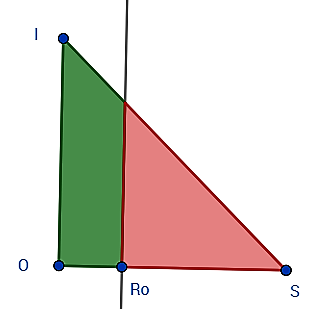
\includegraphics[width=5cm]{images/4MB3_A1_2c.png}
\end{figure}
\end{center}
Consider the relative area, as shown here. First we will examine the green area, written as ${\mathcal O}=\{(-\infty,\frac{1}{{\mathcal R}_o}) \times \mathbb{R}\}\cap \Delta$, where $\Delta=\{(S,I):S\ge0,\, I\ge0,\, S+I\le1\}$ as shown in the image, and ${\mathcal O}$ is an open subset relative to the area of interest. We will also use the closed set ${\mathcal C}=\{[0,\frac{1}{{\mathcal R}_o}-\delta]\times{0}\}, \delta > 0$. As stated previously, any state with $I=0$ will remain in that set, making $\mathcal C$ an invariant set. Knowing this we can now invoke \textit{Lyapunov's Direct Method of Closed Invariant Sets} using the Lyapunov function, $\mathcal{L} = I$. It is easily shown that this is a strict Lyapunov function on $\mathcal{O} \setminus \mathcal{C}$ and $\mathcal{C}$ is asymptotically stable.
\begin{equation}
{\displaystyle {\begin{aligned}
\mathcal{L}&=I \\
\mathcal{L}(X)&=0 \qquad \forall \quad X \in \mathcal{C} \\
\mathcal{L}(X) &> 0 \qquad \forall \quad X \in \mathcal{O} \setminus \mathcal{C} \\
\frac{d\mathcal{L}(X)}{dt} &= \frac{dI}{dt}=I(\mathcal{R}_0 \cdot S-1) \\
\frac{d\mathcal{L}(X)}{dt} &= 0 \qquad \forall \quad X \in \mathcal{C} \\
\frac{d\mathcal{L}(X)}{dt} &< 0 \qquad \forall \quad X \in \mathcal{O} \setminus \mathcal{C}
\end{aligned}}}
\end{equation}
We now conclude that the set of $I=0$ is asymptotically stable for any initial conditions in $\mathcal{O}$.\break
Next we need to show that any trajectories with initial conditions in $\Delta \setminus \mathcal{O}$, in green in the diagram, will eventually land in $\mathcal{O}$ at which point we use the asymptotic stability of $\mathcal{C}$ as we showed above. 
For any point, $P \in \Delta \setminus \mathcal{O}, P=\{(S,I)|S \geq \frac{1}{\mathcal{R}_0}, I > 0, S+I \leq 1\}$. We can see from ~\eqref{E:SIR} that $\frac{dS}{dt} < 0$ for all $P$. This means that $S$ will decrease and continue to decrease until $P \in \mathcal{O}.$
\break
This makes biological sense as any endemic will end eventually, at which point there will be no infectious individuals, so $I=0$. 

\end{proof}
}
\item \basicSIRanalQd

{\color{blue}
\begin{proof}[Solution]
{\color{magenta}\dots beautifully clear and concise text to be inserted here\dots}
\end{proof}
}

\end{enumerate}

\newpage
\section*{Notes on Lyapunov functions}\hypertarget{NotesLyapFuns}{}

\NotesOnLyapunovFunctions

\bibliographystyle{vancouver}
\bibliography{4mba1_2018}

\bigskip

\centerline{\bf--- END OF ASSIGNMENT ---}

\bigskip
Compile time for this document:
\today\ @ \thistime

\end{document}
